\begin{figure}[ht]
  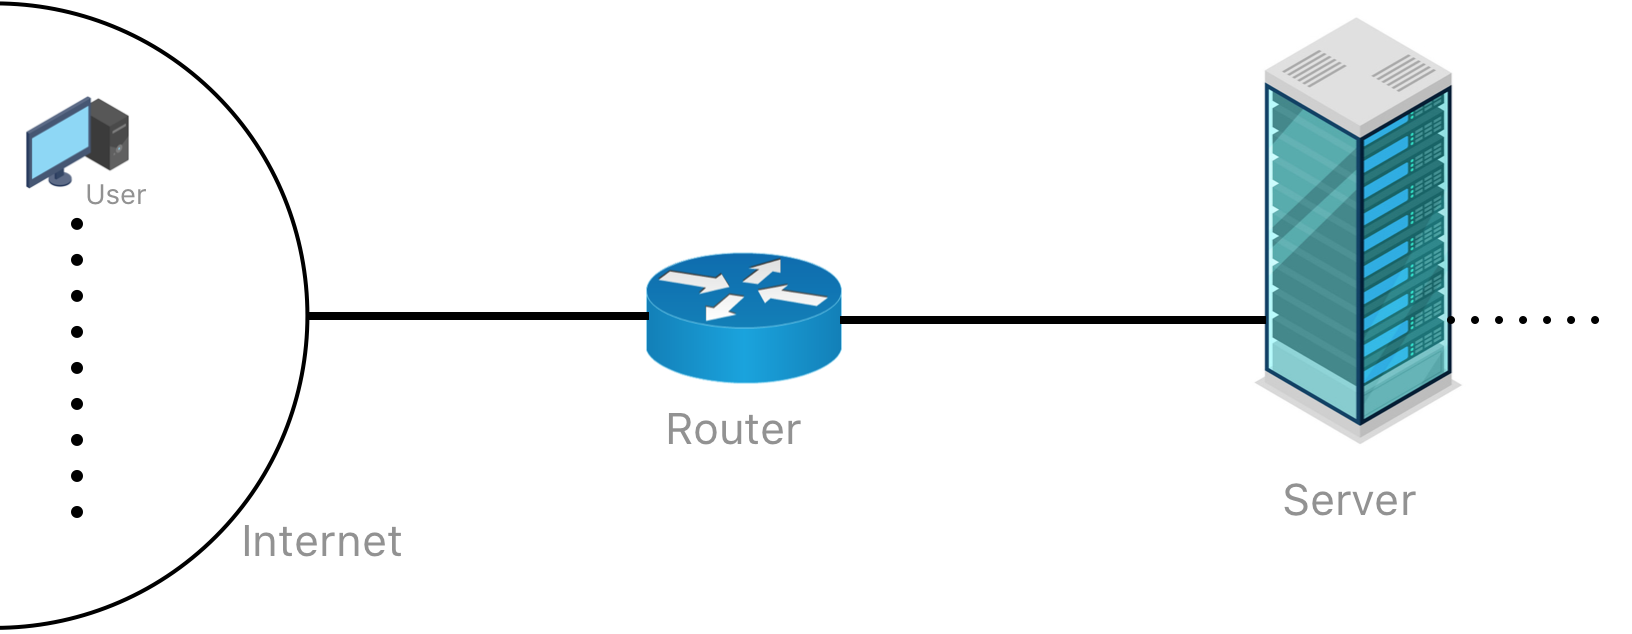
\includegraphics[scale=0.31]{imgs/scenario.png}
  \caption{Network Scenario}
  \label{fig:networkscenario}
\end{figure}

\begin{figure*}[h]
	\begin{subfigure}{0.48\textwidth}
		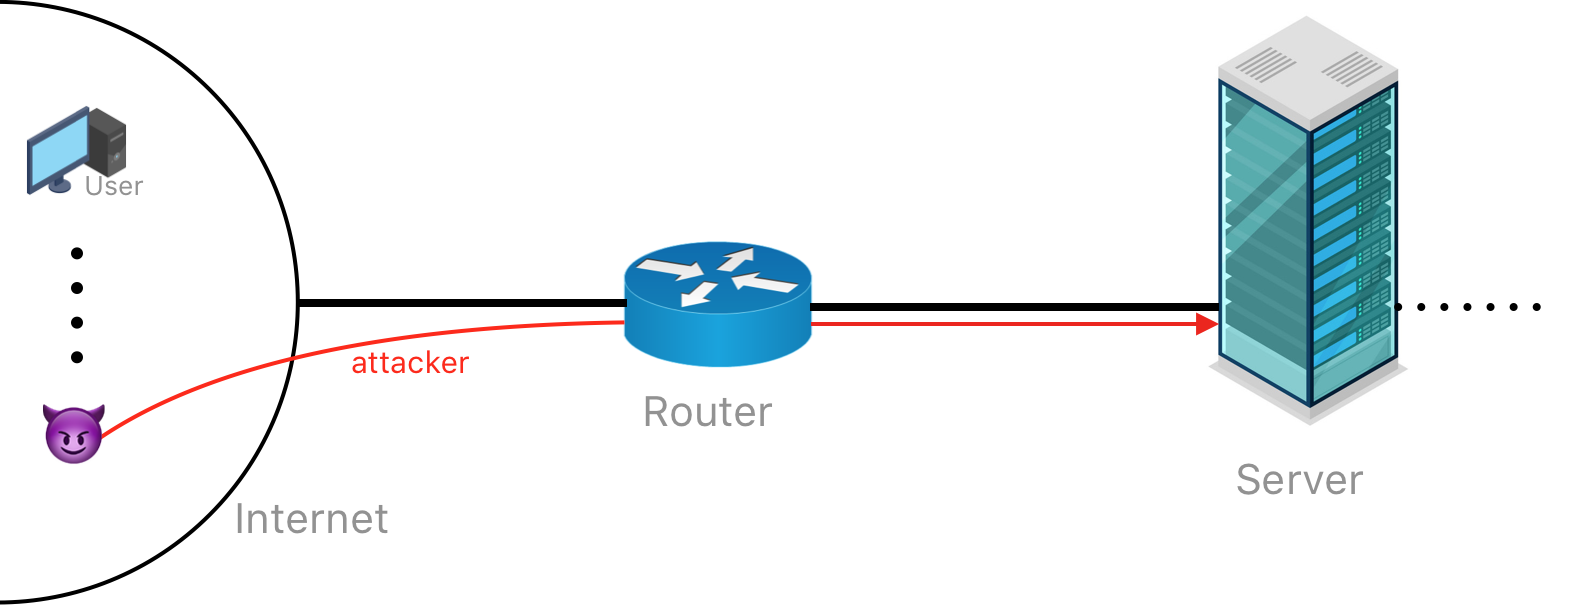
\includegraphics[width=\textwidth]{imgs/DoS_attack.png}
		\caption{DoS attack scenario} \label{fig:DoS}
	\end{subfigure}
	\hspace*{\fill} % separation between the subfigures
	\begin{subfigure}{0.48\textwidth}
		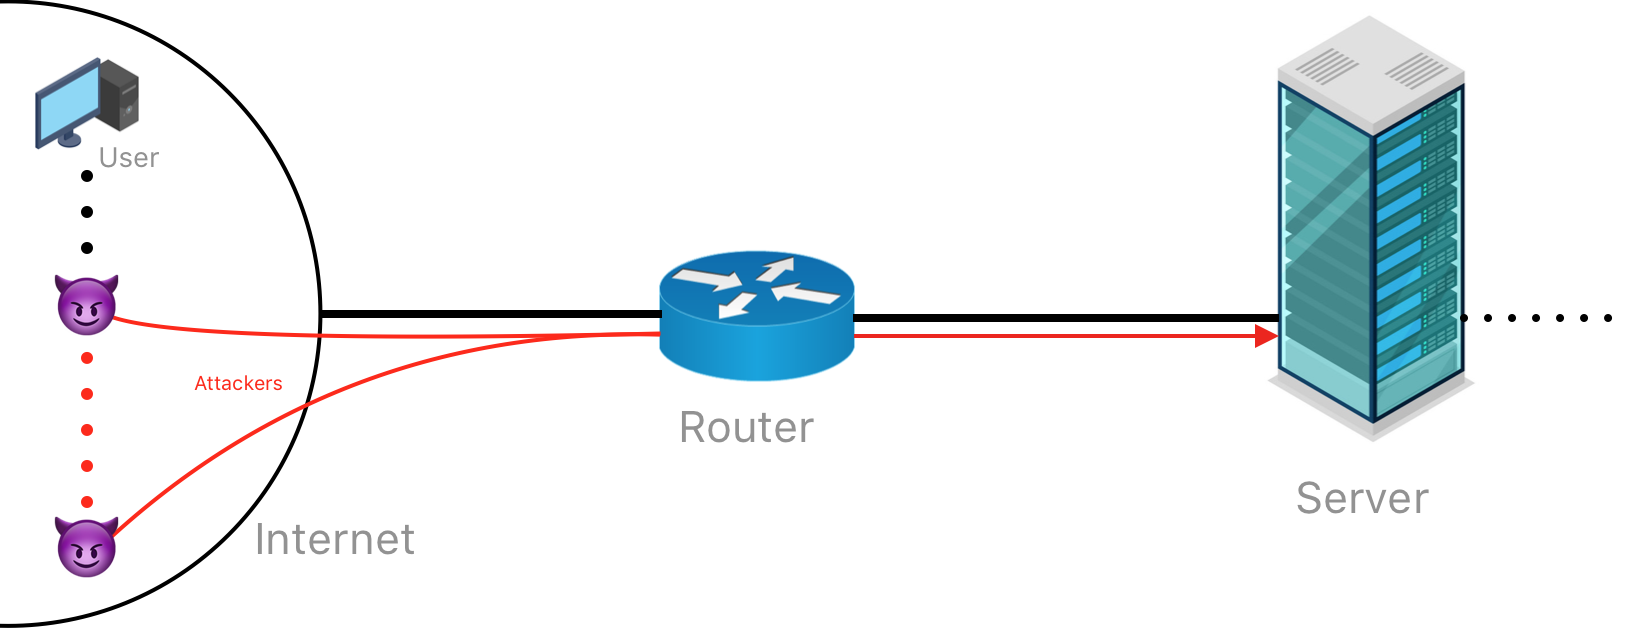
\includegraphics[width=\textwidth]{imgs/DDoS_attack.png}
		\caption{DDoS attack scenario} \label{fig:DDoS}
	\end{subfigure}
	\caption{Attacks scenarios}
	\label{fig:atks}
\end{figure*}

\section{Project structure and implementation}
Our project and its source code is freely downloadable on \href{https://github.com/CristianTuretta/DDoS-Network-Flow-Forensics-Analyser-.git}{Github}. Here, we focused on the UDP flood D(D)oS analysis of pcap records: the goal is to point out good and evil users given a pcap network sniff file converted to csv format. The project is a multi-layered tool which primarily consists in two executable Python 3 scripts:

\subsection{DDoSAnalysis}
\textit{DDoSAnalysis.py} can be used in two different modes, depending on the line parameters used: 
	\begin{itemize}
		\item \textit{-g dataset\_name n\_members n\_lines n\_attackers atk\_volume atk\_duration} \\Generates a random, bogus dataset in the current working directory with the name specified in the second argument, alongside with the number of normal network users specified in \textit{n\_members} argument, the dimension of the dataset (in lines), the number of infected machines, the attack volume (per packet) and its duration. At the end of the generation process, it copies the dataset into the Hadoop File System. We assumed that Hadoop is installed and a folder tree under \path{hdfs://user/your_user/project/input} exists.
		\item \textit{-a dataset\_name} \\ Begin the analysis of the dataset \textit{dataset\_name} using a Pig script. In order to work, the dataset must have been previously copied into the Hadoop input folder, which automatically happens if the dataset is generated using \textit{-g} option. It saves the elaborated dataset under \path{outputs/dataset_name} with an image consisting of a plot of every agent average velocity (Mbps), an attack volume graph and a statistical image which shows the squared margin to mean velocity.
		\item \textit{-anp dataset\_name} \\ It's like the \textit{-a} argument, but it doesn't start Pig analysis. It's used when we have already completed a Pig analysis, and we only want to aggregate data and obtain the plots. 
		\item \textit{-ga dataset\_name n\_members n\_lines n\_attackers atk\_volume atk\_duration} \\ Launches both the generation and the analysis
		\item \textit{-sga dataset\_name n\_members n\_lines n\_attackers atk\_volume atk\_duration} \\ Launches both the generation and the analysis. After generation but before the Pig analysis, it prints an estimation of the dataset dimension, letting the user choose whether to proceed or not.
	\end{itemize}
The script also automatically records infos about performance timing under \path{PerformanceHistory.csv}.

\subsection{PerformanceAnalyser}
\textit{PerformanceAnalyser.py} is used to automatically plot all the infos stored under \path{PerformanceHistory.csv}. It supports two modes:
	\begin{itemize}
		\item \textit{-a img\_name} \\ Stores a plot under the current working directory named \textit{img\_name} of analysis statistics (history of dataset analyzed and time elapsed)
		\item \textit{-g img\_name} \\ Stores a plot under the current working directory named \textit{img\_name} of dataset generation statistics (history of dataset generated and time elapsed)
	\end{itemize}

\textit{PerformanceAnalyser.py} also exposes a method used as a wrapper to call the generation and analysis routines, using a \textbf{CProfile} python module to gain time statistics.

\bigskip
The first two mentioned scripts are the user interface of our tool. However, we have other core scripts which make the generation/analysis possible:

\subsection{DatasetGenerator}
\textit{DatasetGenerator.py} contains the core generation routine of datasets. It generates a pool of innocent IPs and an attackers' one, then it fills line-by-line the dataset with random and bogus informations, extracting random users and attackers. It saves a csv file in the format: \textit{id, time, source\_ip, dest\_ip, protocol, packet\_size, payload}

\subsection{Evaluator} 
\textit{Evaluator.py} exposes the main routine which processes the Pig script output. It computes the mean velocity of all users, and then produces a plot consisting of the velocity of every single user, represented with a blue line, previously calculated by the Pig script (\textit{udpfloodpcap.pig}) and the mean velocity of all users, represented with a red line. The data scientist could distinguish between evil and good users just looking at the deviation from the average. It also plots a volume comparison graph between users and the squared margin to mean velocity.

\subsection{Pig script}
\textit{Udpfloodpcap.pig} calculates the mean velocity of every machine given a dataset in input. This is the core of the analysis tool: it uses Pig Latin mapreduce paradigm. The script loads the dataset, filter the records having UDP protocol, and group them by \textit{(source\_ip, destination\_ip)} tuple. At this point we have to handle a list of \textit{map(tuple, bag)} containing all the corresponding packets sent by a machine. We can then calculate the number of packets (counting the elements in the bag), the total volume exchanged by a particular machine (summing up the corresponding data for each element of the bag) and the mean velocity in bps (using the total volume divided by the max time minus the min time). This is a crucial factor which we use to discriminate good and evil users.
